\documentclass[../../../../Assignments.tex]{subfiles}


\begin{document}
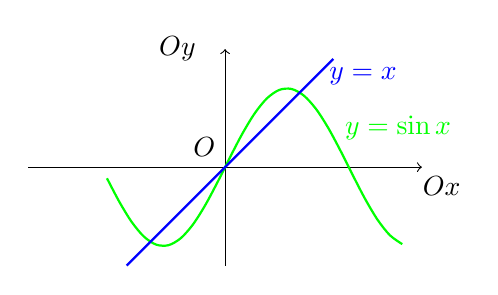
\begin{tikzpicture}[scale=0.5]
    % Oxy
    \draw [<->]   (0,  3  ) -- (0, 0) -- ( 5, 0);
    \draw [black] (0, -2.5) -- (0, 0) -- (-5, 0);
    \node [left] at (-0.5, 3){\(Oy\)};
    \node [below] at (5.5, 0){\(Ox\)};
    \node [left] at (0, 0.5){\(O\)};

    \draw [green, thick, smooth, domain=-3:4.5] plot (\x, {2 * sin(\x r)});
    \node [green, right] at (2.8, 1){\(y = \sin{x}\)};

    \draw [blue, thick, domain=-2.5:2.75] plot (\x, {\x});
    \node [blue, right] at (2.4, 2.3){\(y = x\)};
\end{tikzpicture}
\end{document}
